\chapter{Vergleich der Verifizierung von Implementierungen}

Nachdem im vorigen Kapitel die Spezifikationen und darin verwendete Sprachmittel verglichen wurden,
geht es nun darum zu verifizieren, dass die Implementierungen diese tatsächlich erfüllen.
Die Werkzeuge Verifast bzw. ACSL führen dazu eigene Berechnungen durch, benötigen aber dennoch
zusätzliche Annotationen im Quellcode, damit die korrekten logische Schlüsse gezogen 
werden können. Beispielsweise müssen Schleifeninvarianten ergänzt werden oder sogenannte
Ghost-Commands, die Prädikate oder weitere logische Beweise mit einbeziehen.

\section{Symbolische Ausführung in Verifast}

Die Verifizierung von Implementierungs-Code findet in Verifast über eine symbolische Ausführung statt:
Gestartet wird mit den Vorbedingungen des Methodenvertrags, der Code wird dann wie bei der tatsächlichen
Ausführung von oben nach unten verarbeitet. Jedoch nicht mit konkreten, sondern mit 
abrakten Werten. Diese werden durch logische Formeln repräsentiert, welche die möglichen Variablen-Werte 
beschreiben. Am Ende der Ausführung sind dann bei erfolgreicher Verifizierung alle Voraussetzungen
erfüllt, um die Nachbedingungen direkt abzuleiten.
\newline
\newline
Bei der symbolischen Ausführung werden alle potenziellen Ausführungspfade untersucht: Schleifen
oder auch \texttt{if}-Anweisungen sorgen dafür, dass Verifast diese Verzweigungen einzeln betrachtet
und verifiziert. Existieren z.B. mehrere \texttt{return}-Anweisungen in der Implementierung, so stellt
das Werkzeug sicher, dass in jedem Ausgang die Nachbedingungen gelten.

\begin{SCfigure}[1.7][h!]
	\centering
		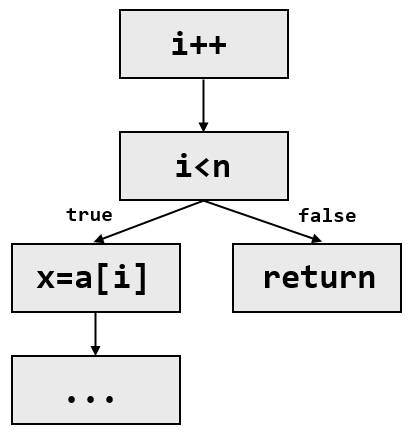
\includegraphics[width=0.3\textwidth]{images/symbolic_execution.png}
		\caption{Ausführungspfade für die symbolische Ausführung einer if-Anweisung}
\end{SCfigure}

Der aktuelle Zustand der Ausführung wird dabei durch zwei verschiedene Strukturen charakterisiert: 
Den Heap, der alle Elemente (engl. heap chunks) des Speichers beinhaltet sowie eine Liste
der geschlussfolgerten Annahmen (engl. assumptions). Bei der Ausführung der Vorbedingungen werden
diese Aussagen nun untersucht und entweder zum Heap hinzugefügt oder zu den Annahmen.

Beim Verstehen dieser Schritte ist die Verifast-Oberfläche sehr hilfreich, da sie den aktuellen
Zustand für einen beliebigen Haltepunkt anzeigen kann. Die folgende Situation zeigt die Ausführung
einer \lstinline{mismatch}-Implementierung bis zum gesetzten Haltepunkt (gelb hervorgehoben).

\begin{center}
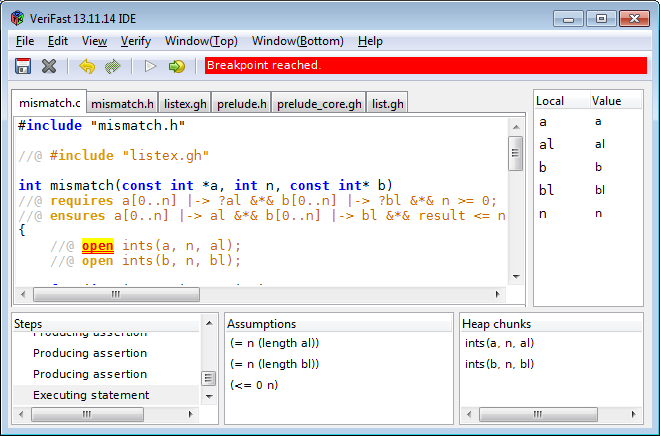
\includegraphics[width=1.0\textwidth]{images/verifast-state-after-precondition.png}
\end{center}

Gut zu erkennen ist, dass logische Ausdrücke wie \(n >= 0\) in die Liste der Annahmen 
(im Bild als \glqq Assumptions\grqq betitelt) aufgenommen wurden. Die \lstinline{ints}-Prädikate hingegen
wurden zum Heap hinzugefügt. Diesen Prozess nennt Verifast \glqq Producing assertion\grqq, wobei sich das Verb
\glqq Producing\grqq auf das Hinzufügen von Elementen zum aktuellen Zustand der symbolischen Ausführung
bezieht.

Das Gegenteil - \glqq Consuming assertion\grqq - findet z.B. beim Verifizieren der Nachbedingungen statt.
Verifast versucht dann alle erforderlichen Aussagen in der Liste der Annahmen bzw. im Heap zu finden
und diese, wenn sie denn passen, zu entfernen. Zusätzlich dazu wird am Ende einer Funktion - beim 
\glqq Leak check\grqq - auch überprüft, dass der Heap (der aktuellen Funktion) leer ist. Ist das nicht 
der Fall so wurde der entsprechende Speicher nicht korrekt bereinigt oder zumindest war Verifast nicht 
in der Lage das Gegenteil zu beweisen.

In dem Fall von mismatch würde Verifast die Heap chunks \lstinline{ints(a, n, al)} sowie
\lstinline{ints(b, n, bl)} beim Konsumieren der Nachbedingung auf dem Heap finden, entfernen und
somit erfolgreich verifizieren können, dass der Speicher so wie vor dem Aufruf vorhanden ist.



\section{Assertions und Ghost-Commands}

Der folgende Quellcode zeigt eine rekursive Implementierung für \lstinline{equal}. Dieser Code
soll als Beispiel für das Erklären der sogenannten Ghost-Commands dienen:

\lstinputlisting[language=C, caption=Rekursive Implementierung für \lstinline{equal} mit Verifast]{codes/equal_recursive_verifast.c}

Ghost-Commands sind Annotationen, die das Werkzeug anweisen Prädikate zu öffnen bzw. zu schließen. Das
ist notwendig, weil Verifast Prädikate auch als Typen behandelt, von denen Instanzen auf dem Heap liegen.

In diesem Beispiel startet die symbolische Ausführung z.B. mit den Prädikaten \lstinline{ints(a, n, al)} 
sowie \lstinline{ints(b, n, bl)} auf dem Heap. Dass die Variable \lstinline{n} tatsächlich die Länge
des Arrays beschreibt ist für Verifast zu dem Zeitpunkt noch nicht erkennbar. Erst das Öffnen über die
Anweisung \lstinline{open ints(a, n, al)} fügt die Inhalte des Prädikats zur Liste der Annahmen hinzu
und entfernt es gleichzeitig vom Heap. Dadurch ist für Verifast ersichtlich, dass \lstinline{n}
gleichzusetzen ist mit \texttt{length(al)} und \texttt{length(bl)}. 

Für die erste \texttt{return}-Anweisung ergibt sich die Annahme \texttt{length(al) = 0} sowie
\texttt{length(bl) = 0} über die Variable \texttt{n}. Damit kann Verifast die Nachbedingung
erfolgreich verifizieren, da eine Liste der Länge 0 gleichzusetzen ist mit dem Konstruktor
\texttt{nil} (siehe dazu \ref{sec:induktive-listen}) und sich der Ausdruck für den Rückgabewert
damit auf \texttt{true == (nil == nil)} reduziert.

Die Umkehroperation - das Schließen eines Prädikats - ist zum Beweisen der Nachbedingung ebenfalls notwendig:
Dabei wird das Prädikat ausgewertet und bei Erfolg wieder auf den Heap gepackt. Dies passiert hier an mehreren 
Stellen ganz automatisch, da es sich bei \lstinline{ints} um ein sogenanntes präzises Prädikat handelt. 
Darunter versteht Verifast Prädikate mit eingehenden und ausgehenden Parametern, die exakt die gleiche 
Speicherregion repräsentieren. 

\begin{figure}[H]
Die Kennzeichnung als präzises Prädikat geschieht über die Nutzung eines Semikolons bei der Trennung
der Prädikaten-Parameter:

\lstinputlisting[language=C, caption=Präzises Prädikat \lstinline{ints}]{codes/ints_precise_predicate_verifast.c}
\end{figure}

Präzise Prädikate versucht Verifast während der Verifizierung automatisch zu öffnen und ggf. auch zu
schließen. Dadurch ist in der obigen Implementierung insbesondere das Schreiben von \texttt{close}-Anweisungen
nicht notwendig.
\newline
\newline
Mit Hilfe der im Quelltext angegebenen Ghost Commands kann Verifast die Implementierung nun erfolgreich
verifizieren.

\section{ACSL-Implementierung im Vergleich}

rekursive implementierung mit acsl zeigen

toolunterstützung frama-c zeigen und erklären

\section{Schleifeninvarianten}

schleifeninvarianten in acsl

alle angefassten variablen müssen per assigns erlaubt werden

dann in verifast zeigen

ähnlich, alles muss in invariante defniiert sein, was man benutzen will

\section{Lemmata und Axiome}

intsinv zeigen mit length

fixpoint nochmal zeigen (take)

erwähnen dass verifast terminierung von fixpount und lemmas prüft

\lstinline{take_one_plus} lemma zeigen

ggf. screenshot hier erst zeigen

erklären wieso es notwendig ist

\section{Speicherprobleme aufdecken}

malloc/free - chunks

zeigen an hand von main-funktion (unit-test)

verifast hilft klar zu dokumentieren wer für speicher verantwortlich ist (rufer oder gerufener)

\section{Überläufe erkennen}

overflow checken
